\documentclass[xcolor=x11names,compress]{beamer}
 
%% General document %%%%%%%%%%%%%%%%%%%%%%%%%%%%%%%%%%
\usepackage[utf8]{inputenc}
\usepackage[english,ngerman]{babel}
\usepackage{graphicx}
\usepackage{color}
\usepackage{tikz}
\usepackage{graphicx}
\usepackage{url}

%%%%%%%%%%%%%%%%%%%%%%%%%%%%%%%%%%%%%%%%%%%%%%%%%%%%%%


%% Beamer Layout %%%%%%%%%%%%%%%%%%%%%%%%%%%%%%%%%%
\useoutertheme[subsection=false,infolines]{miniframes}
\useinnertheme{default}
\usefonttheme{serif}
\usepackage{palatino}

\setbeamertemplate{footline}[frame number]
\setbeamertemplate{caption}[numbered]

\setbeamerfont{title like}{shape=\scshape}
\setbeamerfont{frametitle}{shape=\scshape}

\setbeamercolor*{lower separation line head}{bg=DeepSkyBlue4} 
\setbeamercolor*{normal text}{fg=black,bg=white} 
\setbeamercolor*{alerted text}{fg=red} 
\setbeamercolor*{example text}{fg=black} 
\setbeamercolor*{structure}{fg=black} 
 
\setbeamercolor*{palette tertiary}{fg=black,bg=black!10} 
\setbeamercolor*{palette quaternary}{fg=black,bg=black!10} 

\renewcommand{\(}{\begin{columns}}
\renewcommand{\)}{\end{columns}}
\newcommand{\<}[1]{\begin{column}{#1}}
\renewcommand{\>}{\end{column}}


\beamertemplatenavigationsymbolsempty
\setcounter{tocdepth}{1}

\setbeamercolor{page number in head/foot}{fg=black}
\definecolor{bordeaux}{rgb}{0.71,0.01,0.29}
\definecolor{codebg}{rgb}{0.82,0.82,0.82}
\definecolor{codehighlight}{HTML}{D4772A}

%%%%%%%%%%%%%%%%%%%%%%%%%%%%%%%%%%%%%%%%%%%%%%%%%%


\begin{document}



\begin{frame}[plain]
  \begin{figure}
    \flushright
      
\includegraphics[scale=0.12]{hu_logo}
    \vspace*{-0.4cm}
  \end{figure}

  \title{\textbf{Bosch's CAN bus\\Investigation of the standard}\\\vspace{0.2cm}}

  \author{Meryem Can\\Stephan Fahrenkrog-Petersen\\Jakob Rüßler\\Thomas Schlegel\\
  Daniel Titz\\Duc Anh Tran\\\vspace{0.3cm}}

\selectlanguage{english}

\date{\today}
\titlepage
\end{frame}


\section{\scshape Introduction}
\begin{frame}
  \frametitle{Introduction and Basic Concepts}
  \begin{itemize}
      \item Controller Area Network~\cite{can}
      \item Serial communications protocol/bus system
      \item Supports distributed realtime control with a very high level of security 
   
  \end{itemize}

\end{frame}


\begin{frame}
  \frametitle{Purpose and Context }
  \begin{itemize}
      \item Created by BOSCH
      \item Used automotive industry 
      \item Automotive electronics, engine control units, sensors, anti-skid-systems
      \item High speed networks to low cost multiplex wiring
  \end{itemize}

\end{frame}

\begin{frame}
  \frametitle{Related standards}
  \begin{itemize}
      \item standardized after ISO 11898
      \item ISO 11898-2 (Highspeed-CAN) - related
      \item ISISO 11898-3 (Lowspeed-CAN)- related      
      \item Not compatible with each other
  \end{itemize}

\end{frame}

%\begin{frame}
%  \frametitle{higher standards}
%  \begin{itemize}
%      \item 
%      \item 
%      \item     
%      \item 
%  \end{itemize}
%
%\end{frame}

\section{\scshape Messages}
\begin{frame}
  \frametitle{Message Transfer and Validation -- 1}
  Overview:
  \begin{itemize}
    \item Information is sent in fixed format messages of different but limited lengths
    \item When free, any connected unit may send messages over the bus
    \item The content of the message is named by an identifier
  \end{itemize}

\end{frame}

\begin{frame}
  \frametitle{Message Transfer and Validation -- 2}
  
    \centering
    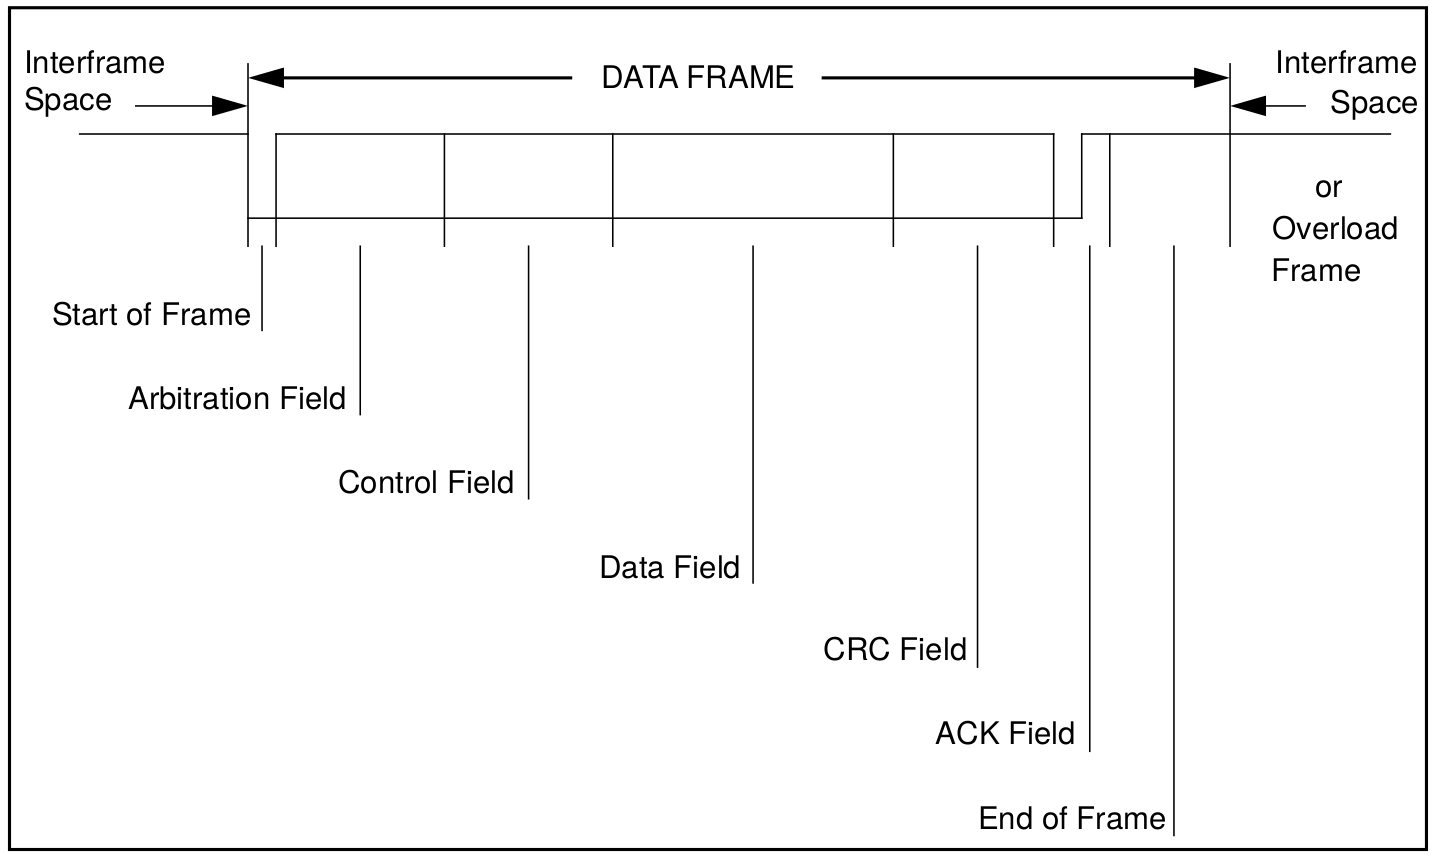
\includegraphics[scale=0.2]{framesetup}

\end{frame}


\begin{frame}
  \frametitle{Message Transfer and Validation -- 3}
  
  \begin{itemize}
    \item Multi-master serial bus standard
    \item All nodes in the network need to be synchronized
    \item ``Dominant'' and ``recessive'' bits
  \end{itemize}

\end{frame}



\section{\scshape Coding / Errors}
\begin{frame}
  \frametitle{Coding and Error Handling -- 1}

  Overview:
  \begin{itemize}
    \item Bit stuffing $\rightarrow$ control mechanism
    \item Distortions etc. $\rightarrow$ error handling to achieve error tolerance
    \item 5 different error types (Bit, Stuff, CRC, Form, ACK)
  \end{itemize}

\end{frame}

\begin{frame}
  \frametitle{Coding and Error Handling -- 2}

  \begin{itemize}
    \item Message passing mechanism, no additional structure needed
    \item Errors broadcasted when detected
    \item Semantics important for correct transmission
    \item Drivers: reliability, error limitation
    \item Problem: new error types?
  \end{itemize}

\end{frame}


\section{\scshape Fault Confinement}
\begin{frame}
  \frametitle{Fault Confinement}
  
    \begin{itemize}
    \item Unit can have 3 states and 2 counters
    \item Strength: Enables extensibility
    \item Drivers: Seperation of concern, reliability, error limitation
    \item Problem: More Unit means more errors?
  \end{itemize}

\end{frame}


\section{\scshape Bit Timing}
\begin{frame}
  \frametitle{Bit Timing Requirements}


\begin{itemize}
    \item List of definitions and rules
    \item Strength: short, but includes everything important
    \item Weaknesses: almost text only, hard to read (structure),
        like a glossary
    \item Improvable by usage of more pictures and examples

\end{itemize}


\end{frame}


\section{\scshape CAN Oscillator}
\begin{frame}
  \frametitle{CAN Enhancement -- 1}

\textbf{Aim:} Increase Oscillator Tolerance
\vspace{0.3cm}

\textbf{Modifications:}
\begin{itemize}
    \item Delay START OF FRAME (SOF) by fully sample INTERMISSION
    \item Insert (not necessary) OVERLOAD FRAME
    \item Synchronise on recessive to dominant edges
\end{itemize}

\end{frame}

\begin{frame}
  \frametitle{CAN Enhancement -- 2}
Still valid:
\begin{itemize}
    \item Hard Sync on SOF 
    \item No SOF until three recessive Bits on INTERMISSION have been read
\end{itemize}

What was achieved?
\begin{itemize}
  \item Use of ceramic oscillators instead of quartz oscillators $\rightarrow$~PRICE!
  \item But\ldots all nodes need to work with the enhanced protocol AND only if the most demanding node works with high tolerance
\end{itemize}

\end{frame}

\section{\scshape Conclusion}

\begin{frame}
  \frametitle{Conclusion -- Standard}

\begin{itemize}
 \item CAN: serial bus system with security features by Bosch
 \item Developed for automotive industry
 \item Standalone standard ISO 11898
\end{itemize}

\end{frame}

\begin{frame}
  \frametitle{Conclusion -- Documentation}

\begin{itemize}
 \item Describes CANs technical details
 \item Strengths: compact, covers standard as a whole
 \item Weaknesses: very general, very dry
 \item Improvements: extend by examples, pictures, applications 

\end{itemize}

\end{frame}

\begin{frame}
  \frametitle{Conclusion -- Structure}

\begin{itemize}
 \item Message-passing pattern with multi-master
 \item Strict message semantics to avoid errors

\end{itemize}

\end{frame}

\begin{frame}
  \frametitle{Conclusion -- Properties and Tradeoffs}
\begin{itemize}
 \item Drivers: real time, error handling and limitation, controlled messaging
 \item Tradeoffs: new error types?, error scaling?
\end{itemize}

\end{frame}

\begin{frame}
  \frametitle{References}
  \scriptsize
  \bibliographystyle{unsrt}
  \bibliography{references}
\end{frame}

\end{document}
